\documentclass{article}

\usepackage{graphicx}
\usepackage[backend=bibtex]{biblatex}

\graphicspath{{./images/}}

\addbibresource{sources.bib}


\begin{document}

\begin{titlepage}
	\begin{center}
		\vspace*{1cm}
		
		\textbf{Report on proposed development plans for Flamingoville}
		
		\vspace{1.5cm}
		
		\textbf{Prepared for:}
		
		Mr Jacob de Wet
		
		Flamingoville Town Council
		
		\vspace{1.5cm}
		
		\textbf{Prepared by:}
		
		Mr Jason Russell
		
		Environmentally-aware expert
		
		\vspace{1.5cm}

		\textbf{Key Words:}
		Development, expansion, feasibility
		
		\vspace{1.5cm}
		September 2015
		
	\end{center}
\end{titlepage}
\thispagestyle{empty}

\pagenumbering{roman}
\setcounter{page}{0}

\newpage
\section*{Terms of reference}
In September 2015, Mr Jacob de Wet, a member of the Flamingoville Town Council, initiated this development. The need for it arose as Flamingoville is current unable to accommodate a large influx of annual visitors and a growing labor force of nearby mines. The Council is forced to develop in the lagoon area as there is no other suitable land available.

\paragraph{}

Mr Jacob's specific instructions were the following:

\begin{enumerate}
	\item Examine three proposed development plans given to the Town Council.
	\item Gather information about the existence and location of birds, flora and fauna in the area.
	\item For each plan:
	\begin{enumerate}
		\item Describe the effect of the development as a whole on the marine life of the lagoon itself and its tributary streams and beaches, and describe the counter measures suggested.
		\item Describe the economic and visual impact (aesthetics) of the development on the town and the nature reserve, incorporating the point of view of Flamingoville town residents.
	\end{enumerate}
	\item Draw conclusions on the basis of all the findings and recommend the plan that will do the least damage, and that will have the most positive long term impact on the area.
\end{enumerate}

\newpage
\section*{Executive Summary}

\newpage
\tableofcontents

\pagenumbering{arabic}
\setcounter{page}{0}

\newpage
\section{INTRODUCTION}
\subsection{Subject of and motivation for report}
This report concerns the further development of Flamingoville and the effect of development on the town and nearby nature reserve.

\subsection{Background to investigation}
The Flamingoville Town Council needs to extend the town. The extension is needed in order to accommodate the large influx of annual visitors as well as the growing labor force which has been attracted to Falmingoville because of the mining in the area. Three development plans have been proposed, one of which is to be realized. Due to the lack of suitable develop-able land, the Council is forced to develop in the lagoon area. Flamingoville Town Council member Mr Jacob de Wet has commissioned this report in order to assist in the decision making process.

\subsection{Objectives of report}
The objectives of this report are therefor to:
\begin{itemize}
	\item report on the existence and location of flora and fauna in the development area
	\item consider the effect on marine life and counter measures and describe the economic and aesthetic impact of development for each development plan
	\item draw conclusions based on the findings
	\item make recommendations as to which development plan to implement based on least damge and most positive long term impact
\end{itemize}

\subsection{Limitations and scope of investigation}
This investigation will consider the economic impact of development at a high level only. The cost of additional infrastructure will not be considered.

\subsection{Plan of development}
The report begins by detailing the existence and location of wildlife species in and around the development zone. Thereafter, the effect on marine life as well as the economic and aesthetic impacts of development on the area will be considered for each of the three development plans. Conclusions are then drawn on the basis of these findings and finally, recommendations are made, based on these conclusions.

\newpage
\section{METHOD OF INVESTIGATION}
\subsection{Interviews with local residents}
Residents were privately interviewed. These interviews were semi-structured.

\subsection{Interviews with business owners}
Business owners were privately interviewed. These interviews were semi-structured.

\subsection{Interview with environmental scientist}
Environmental scientist Professor Thabo Ntuli was interviewed.

\subsection{Interview with urban and regional town planner}
Urban and regional town planner Mr Duncan Greenspan was interviewed.

\newpage
\section{EXISTENCE AND LOCATION OF WILDLIFE}
This section concerns the existence and location of wildlife within the development zone.

\begin{figure}[h!]
	\centering
	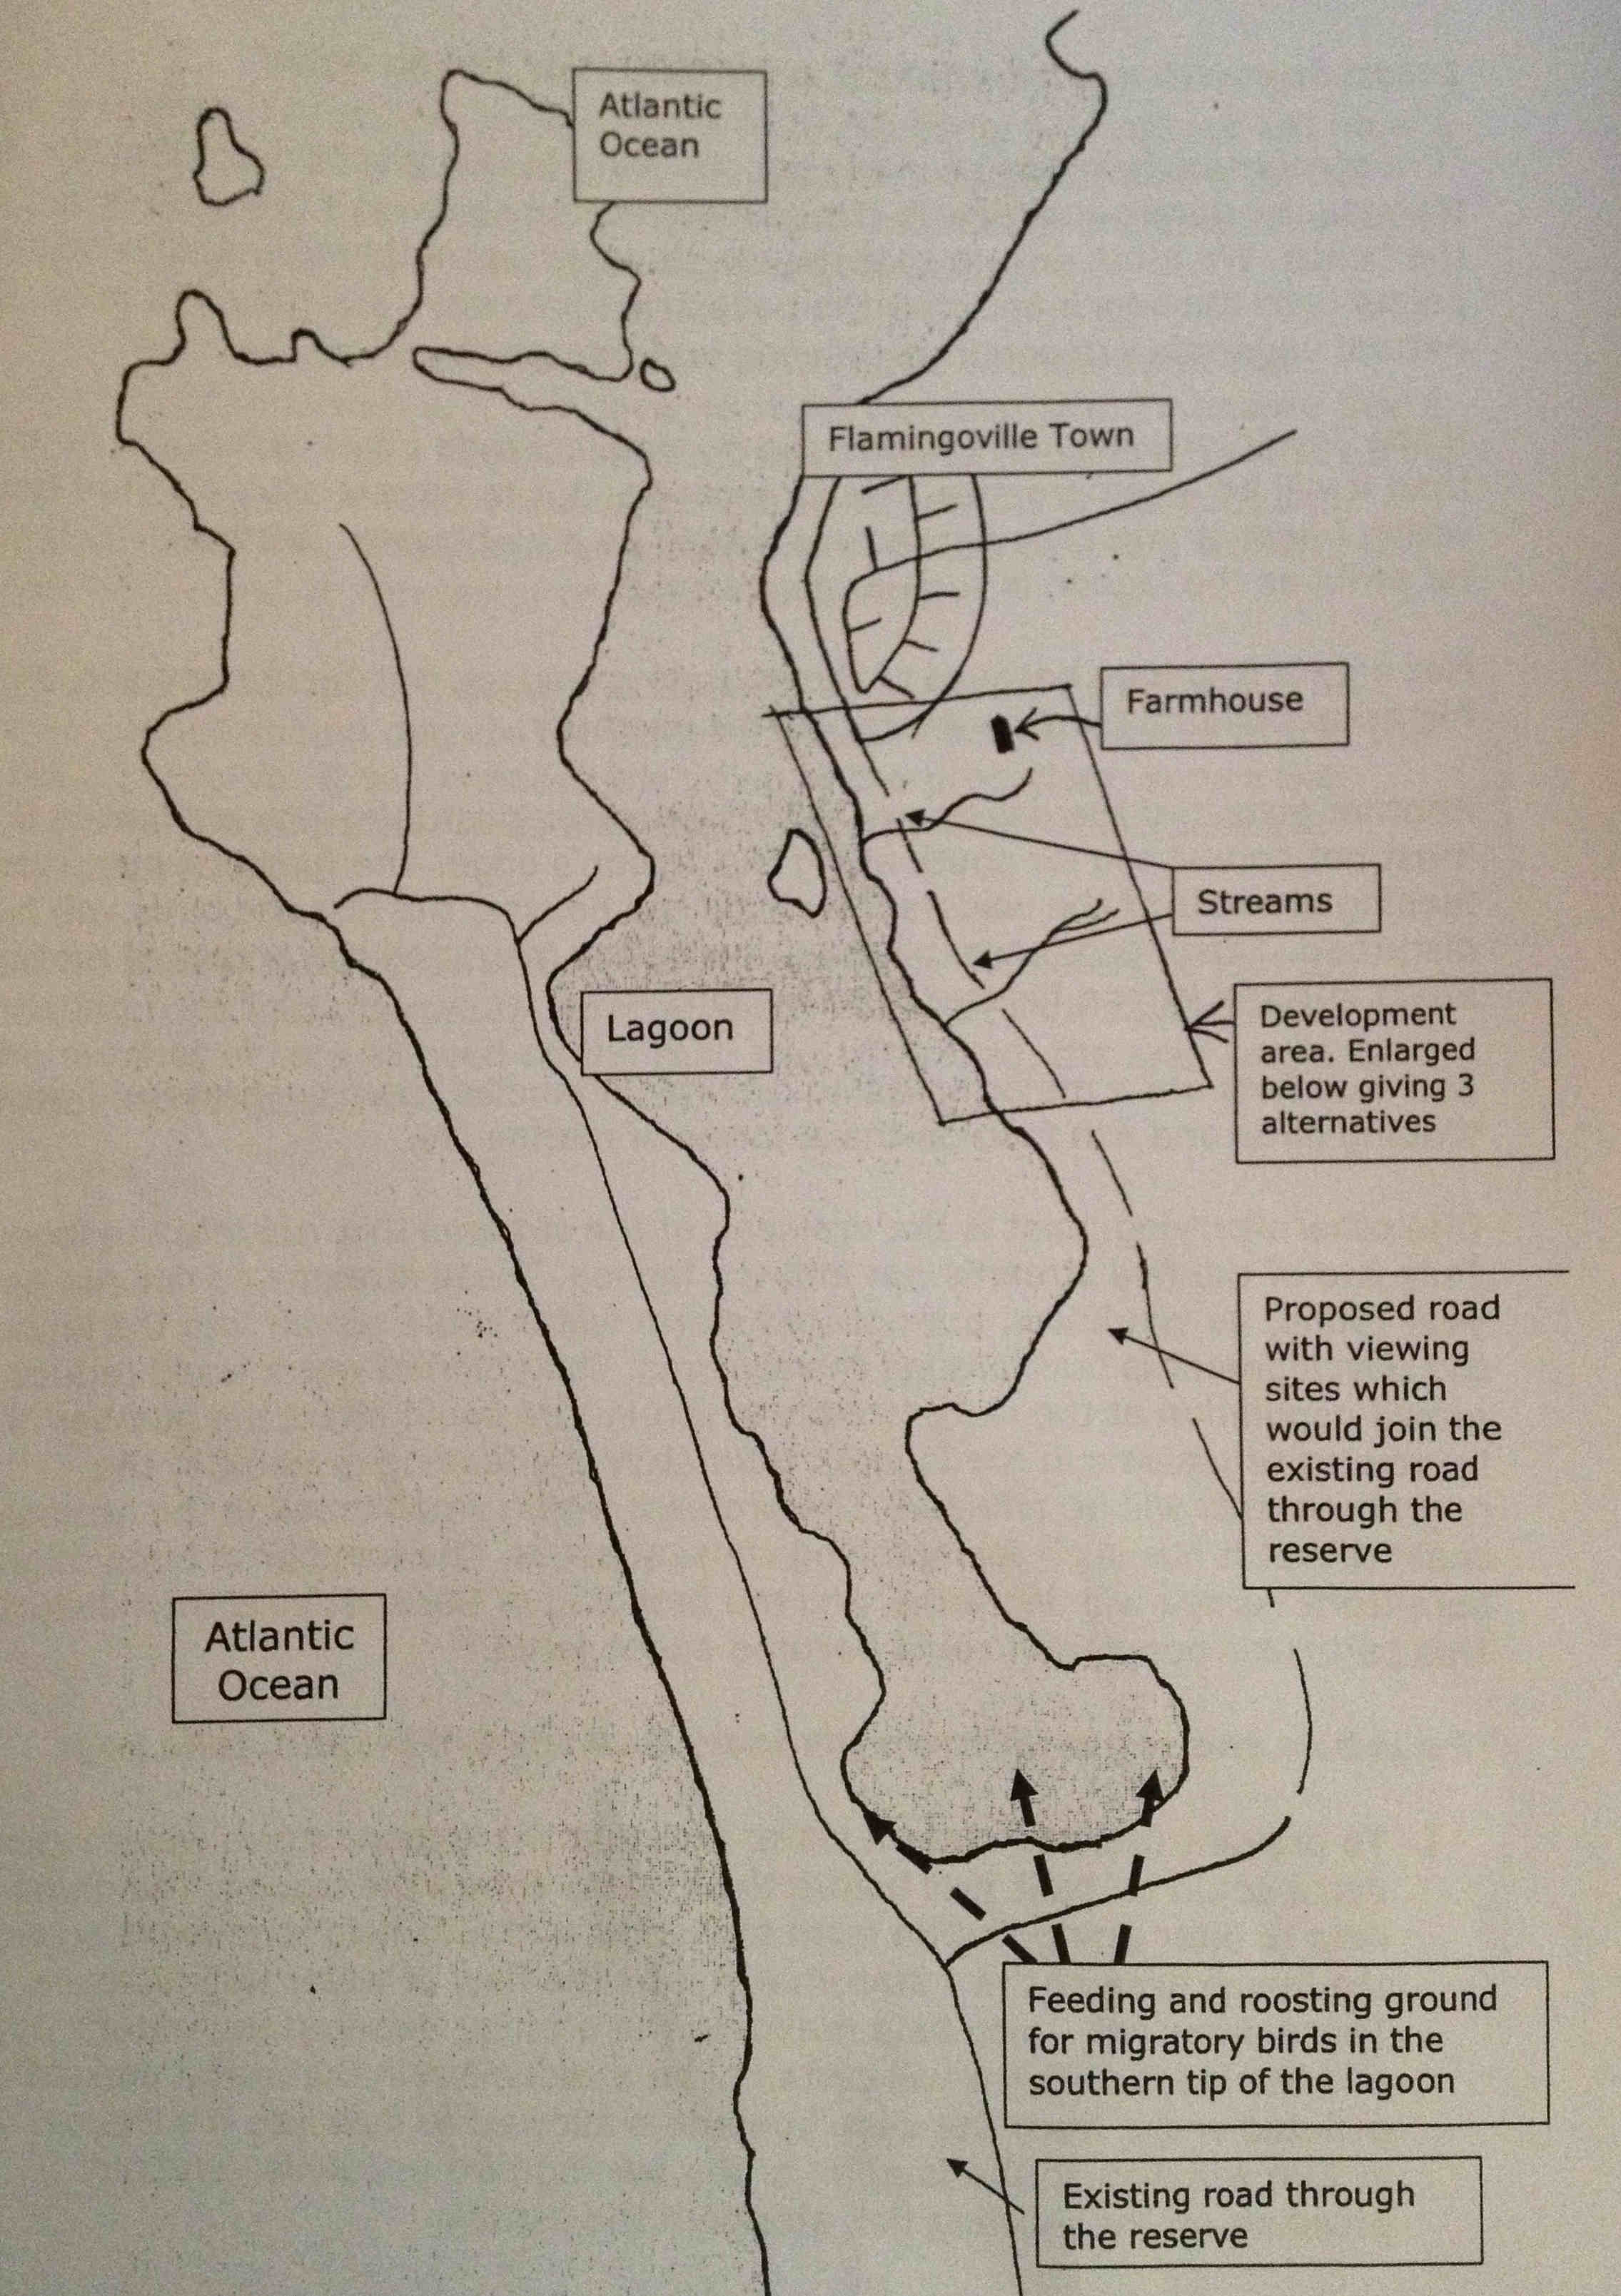
\includegraphics[width=0.6\textwidth]{map}
	\caption{Map of the area}
\end{figure}

\subsection{Flora}
Large portions of the development zone and surrounds is covered in indigenous fynbos. There is also a large variety of wild flowers which bloom in the spring. The fynbos and wild flower species are ubiquitous throughout the region.

\subsection{Fauna}
A protected tortoise species is known to inhabit the area around the development zone. Small buck have also been spotted. Migratory birds feed and roost along the southern tip of the lagoon. The mud flats around the lagoon are also home to welks, clams, worms and prawns. Many fish species exist in the lagoon.

\newpage
\section{EXAMINATION OF PLAN A}
This section concerns the effect on marine life as well as the visual and economic impact of plan A.

\begin{figure}[h!]
	\centering
	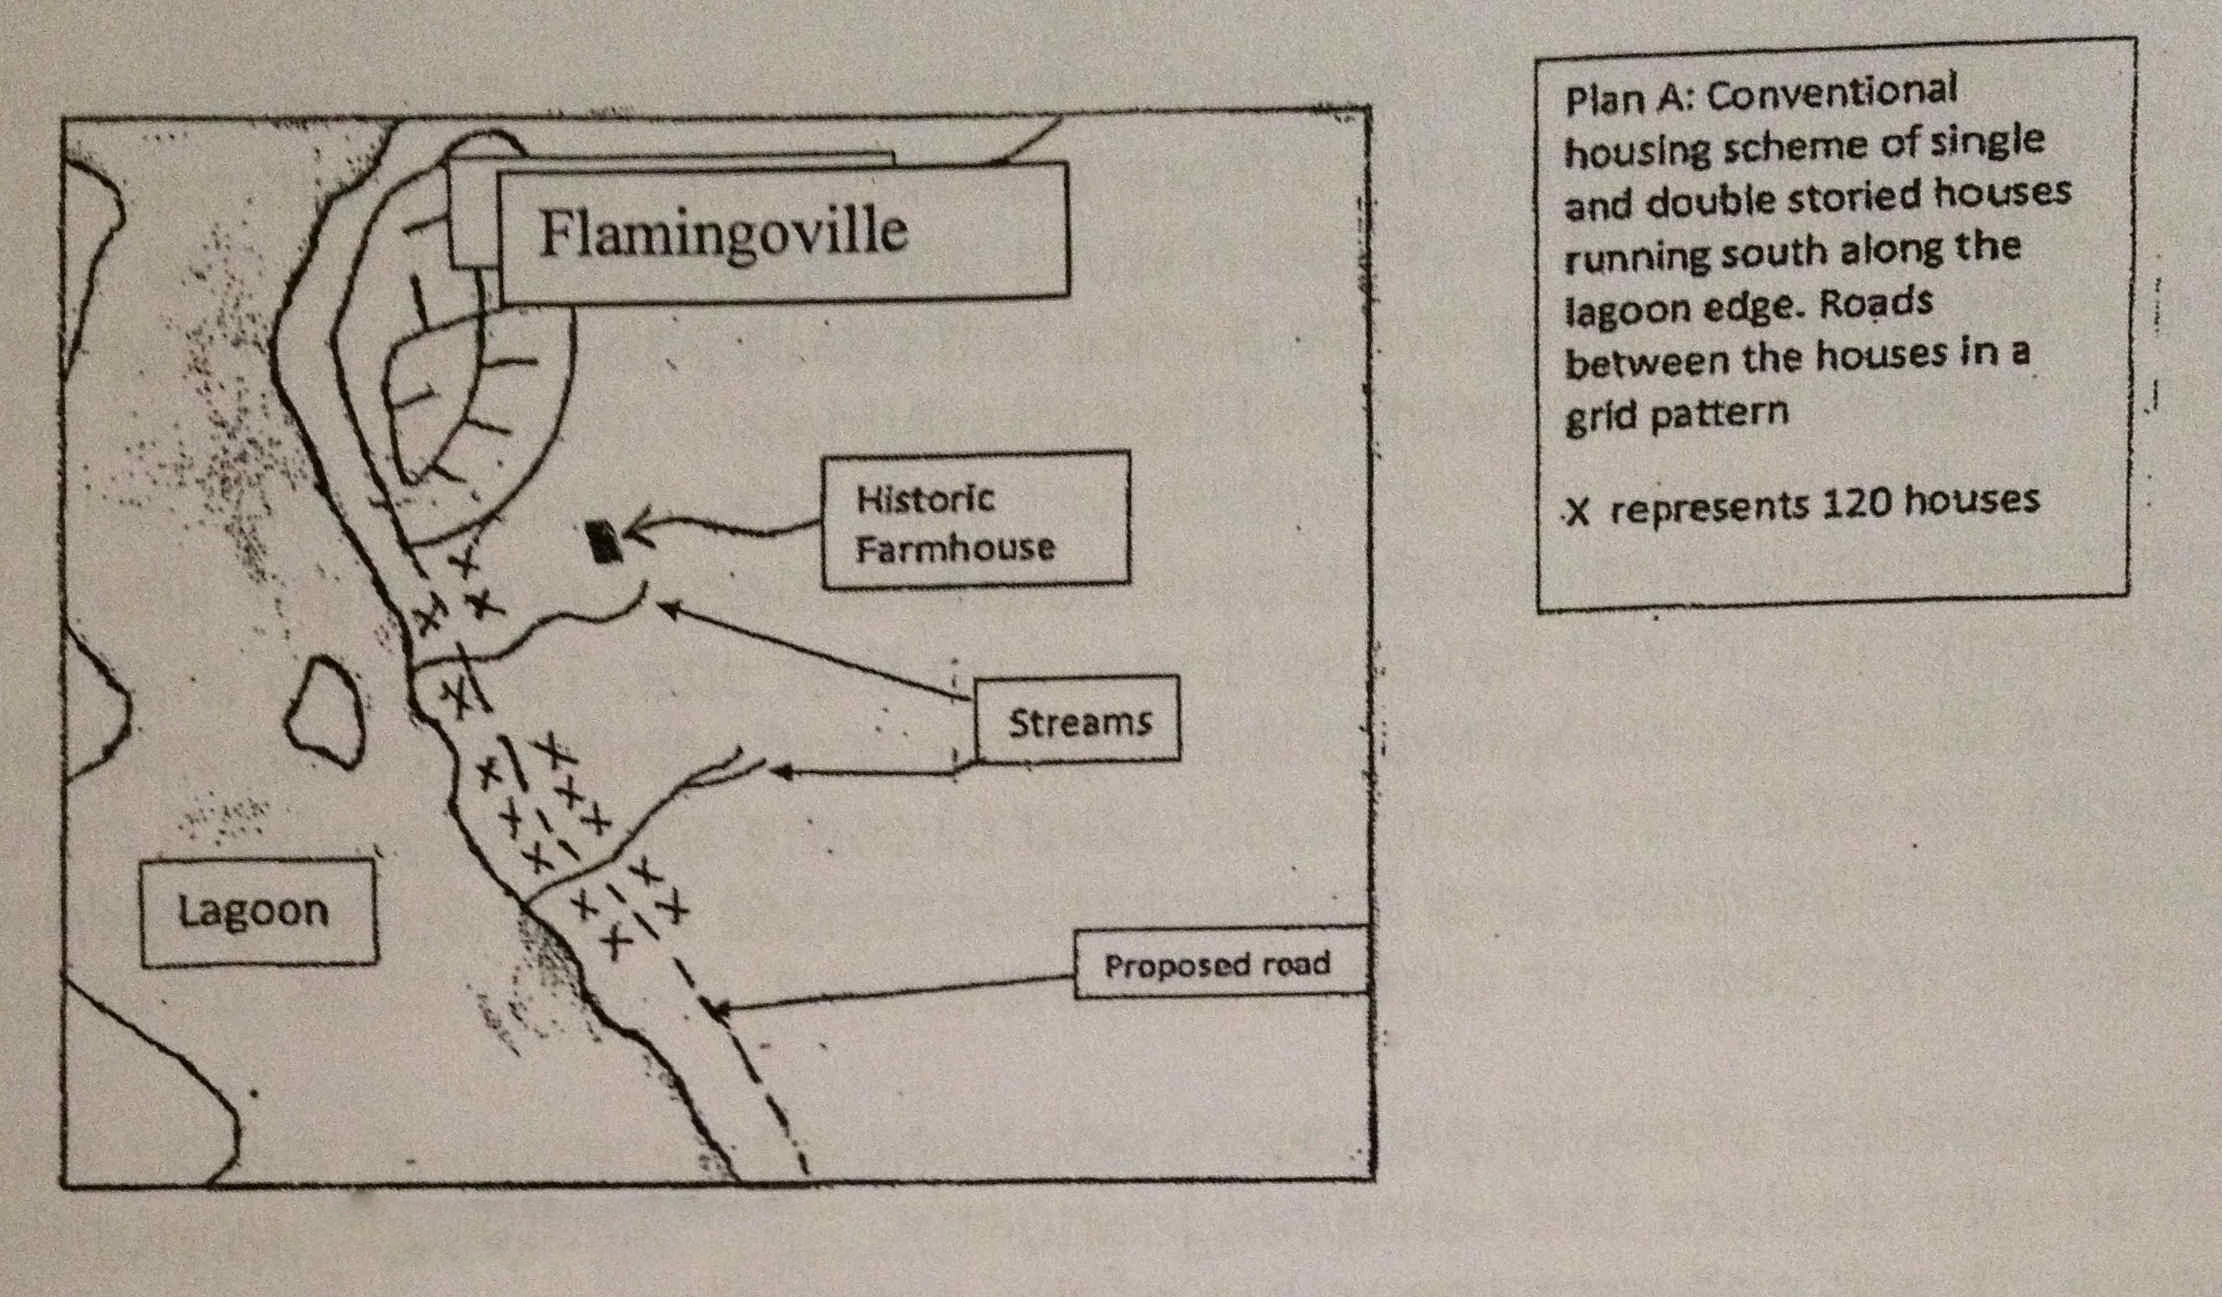
\includegraphics[width=0.6\textwidth]{plan_a}
	\caption{Map of plan A}
\end{figure}

\subsection{Effect on marine life}
\subsubsection{Effect}
\begin{itemize}
	\item A large portion of the lagoon is exposed to development.
	\item Both streams are exposed to development.
\end{itemize}

\subsubsection{Counter measures}
\begin{itemize}
	\item Water retention dams will be constructed to minimize pollution and maintain ecology.
\end{itemize}

\subsection{Economic impact}
\begin{itemize}
	\item The average distance from each house to the center of town is relatively high.
	\item This high distance drives up costs of infrastructure.
	\item Property values will be high as a result of proximity of many houses to lagoon.
\end{itemize}

\subsection{Visual impact}
\begin{itemize}
	\item Double story houses will be constructed.
	\item No development near historic farmhouse.
	\item View from proposed road will be inhibited by neighboring houses.
	\item Large portion of lagoon exposed to development.
\end{itemize}

\newpage
\section{EXAMINATION OF PLAN B}
This section concerns the effect on marine life as well as the visual and economic impact of plan B.

\begin{figure}[h!]
	\centering
	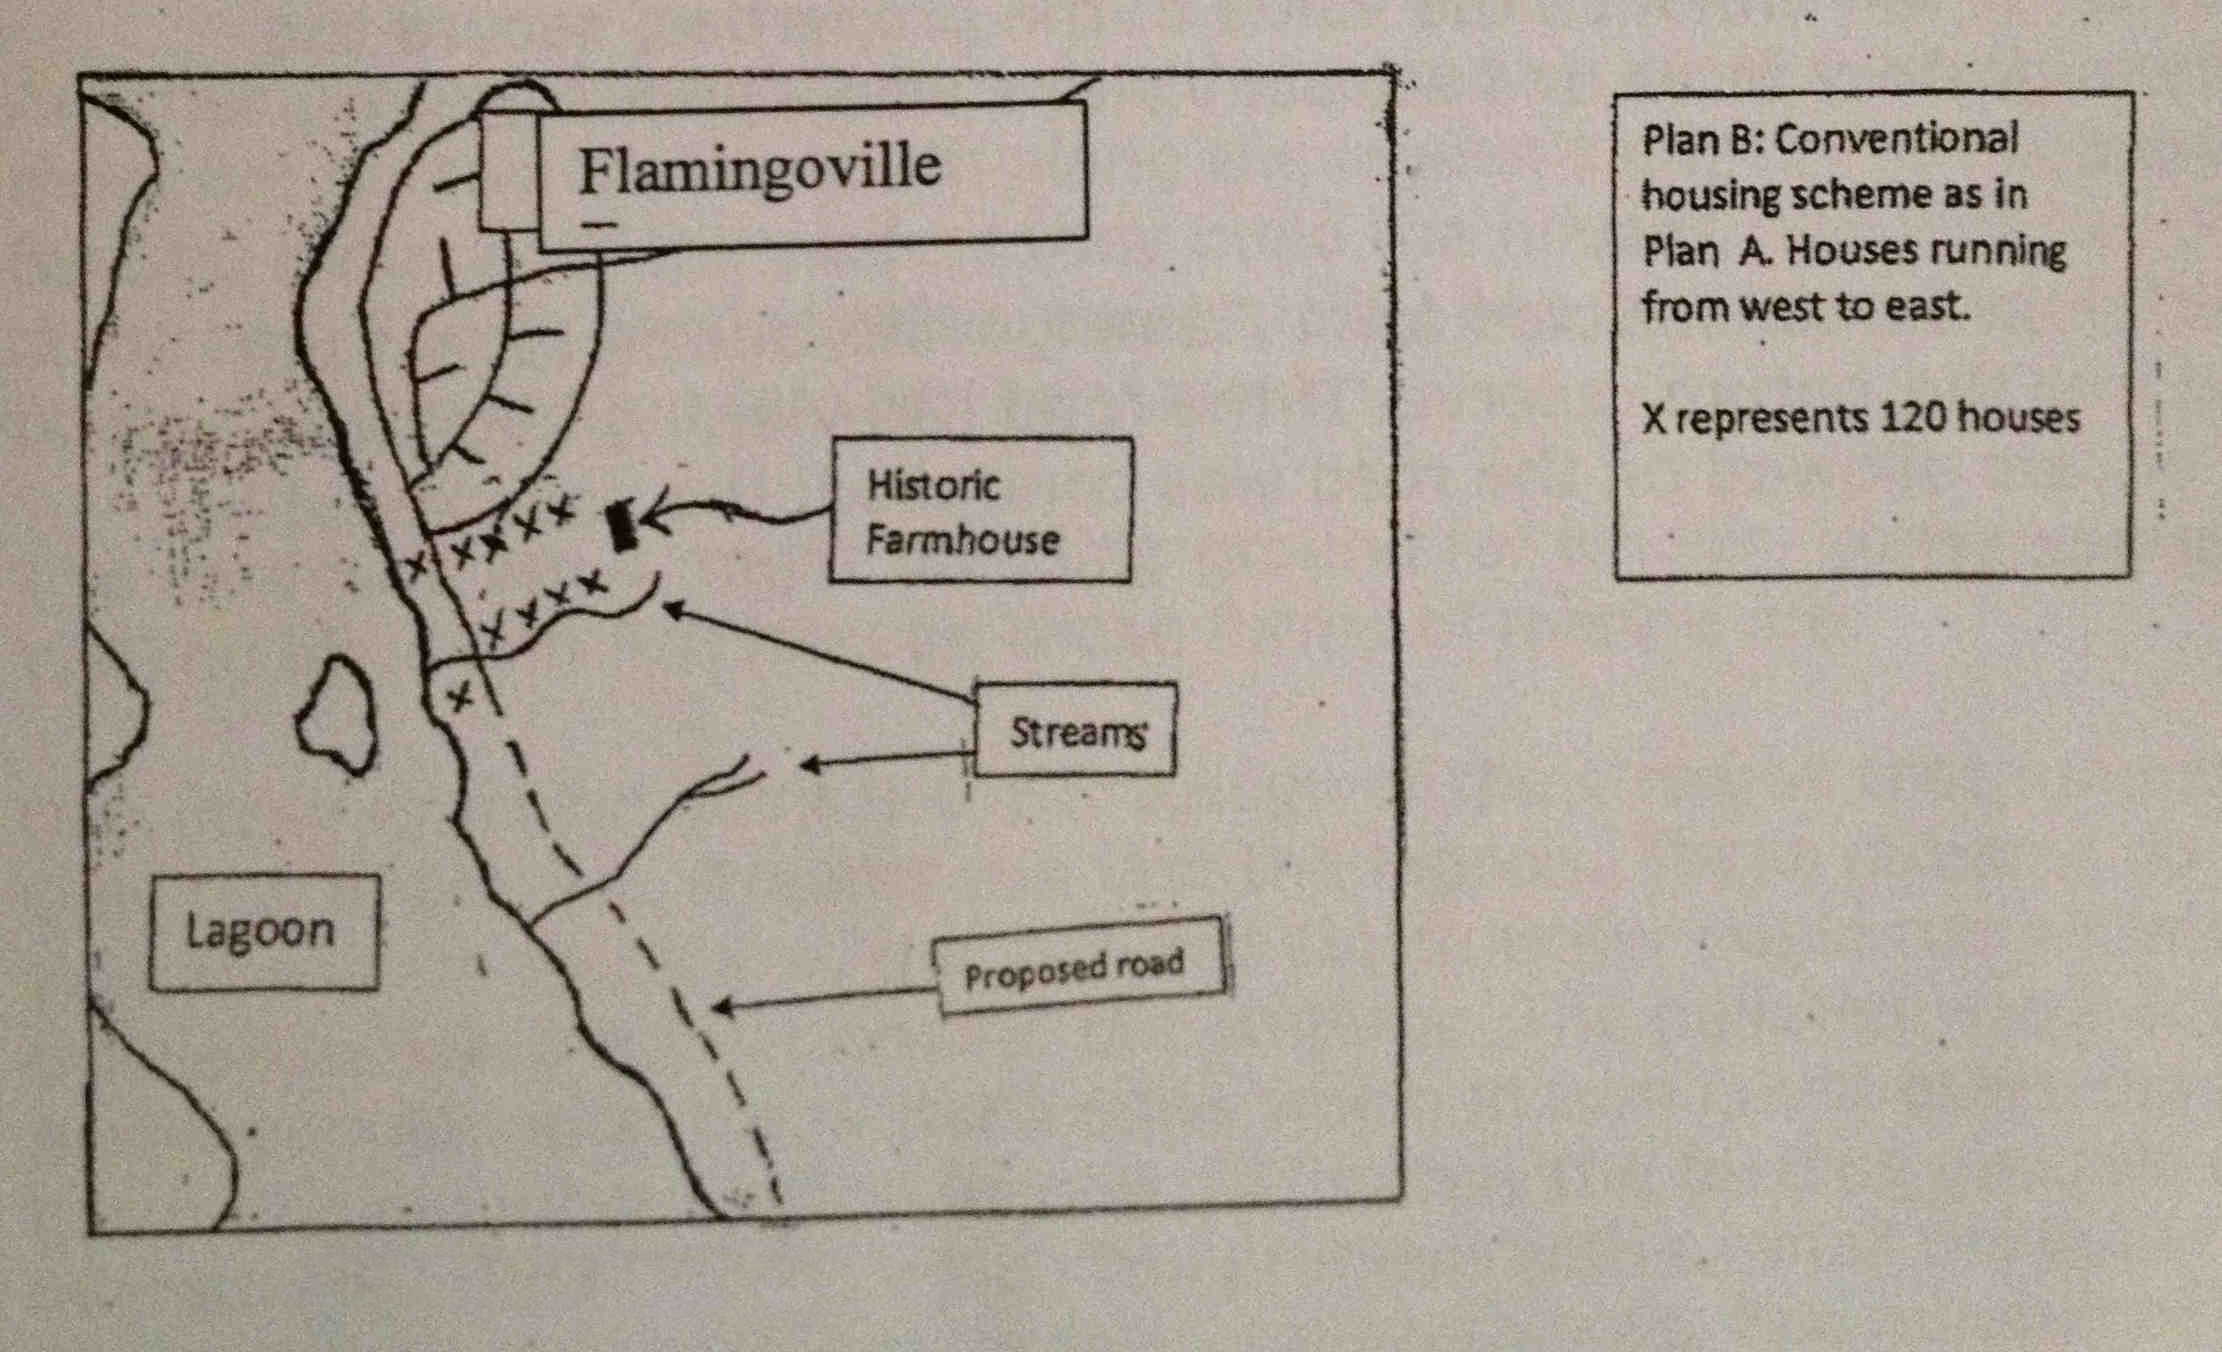
\includegraphics[width=0.6\textwidth]{plan_b}
	\caption{Map of plan B}
\end{figure}

\subsection{Effect on marine life}
\subsubsection{Effect}
\begin{itemize}
	\item A small portion of the lagoon is exposed to development.
	\item Just one stream is exposed to development.
\end{itemize}

\subsubsection{Counter measures}
\begin{itemize}
	\item Water retention dams will be constructed to minimize pollution and maintain ecology.
\end{itemize}

\subsection{Economic impact}
\begin{itemize}
	\item The average distance from each house to the center of town is relatively low.
	\item This low distance drives down costs of infrastructure.
\end{itemize}

\subsection{Visual impact}
\begin{itemize}
	\item Double story houses will be constructed.
	\item Development is near historic farmhouse.
\end{itemize}

\newpage
\section{EXAMINATION OF PLAN C}
This section concerns the effect on marine life as well as the visual and economic impact of plan C.

\begin{figure}[h!]
	\centering
	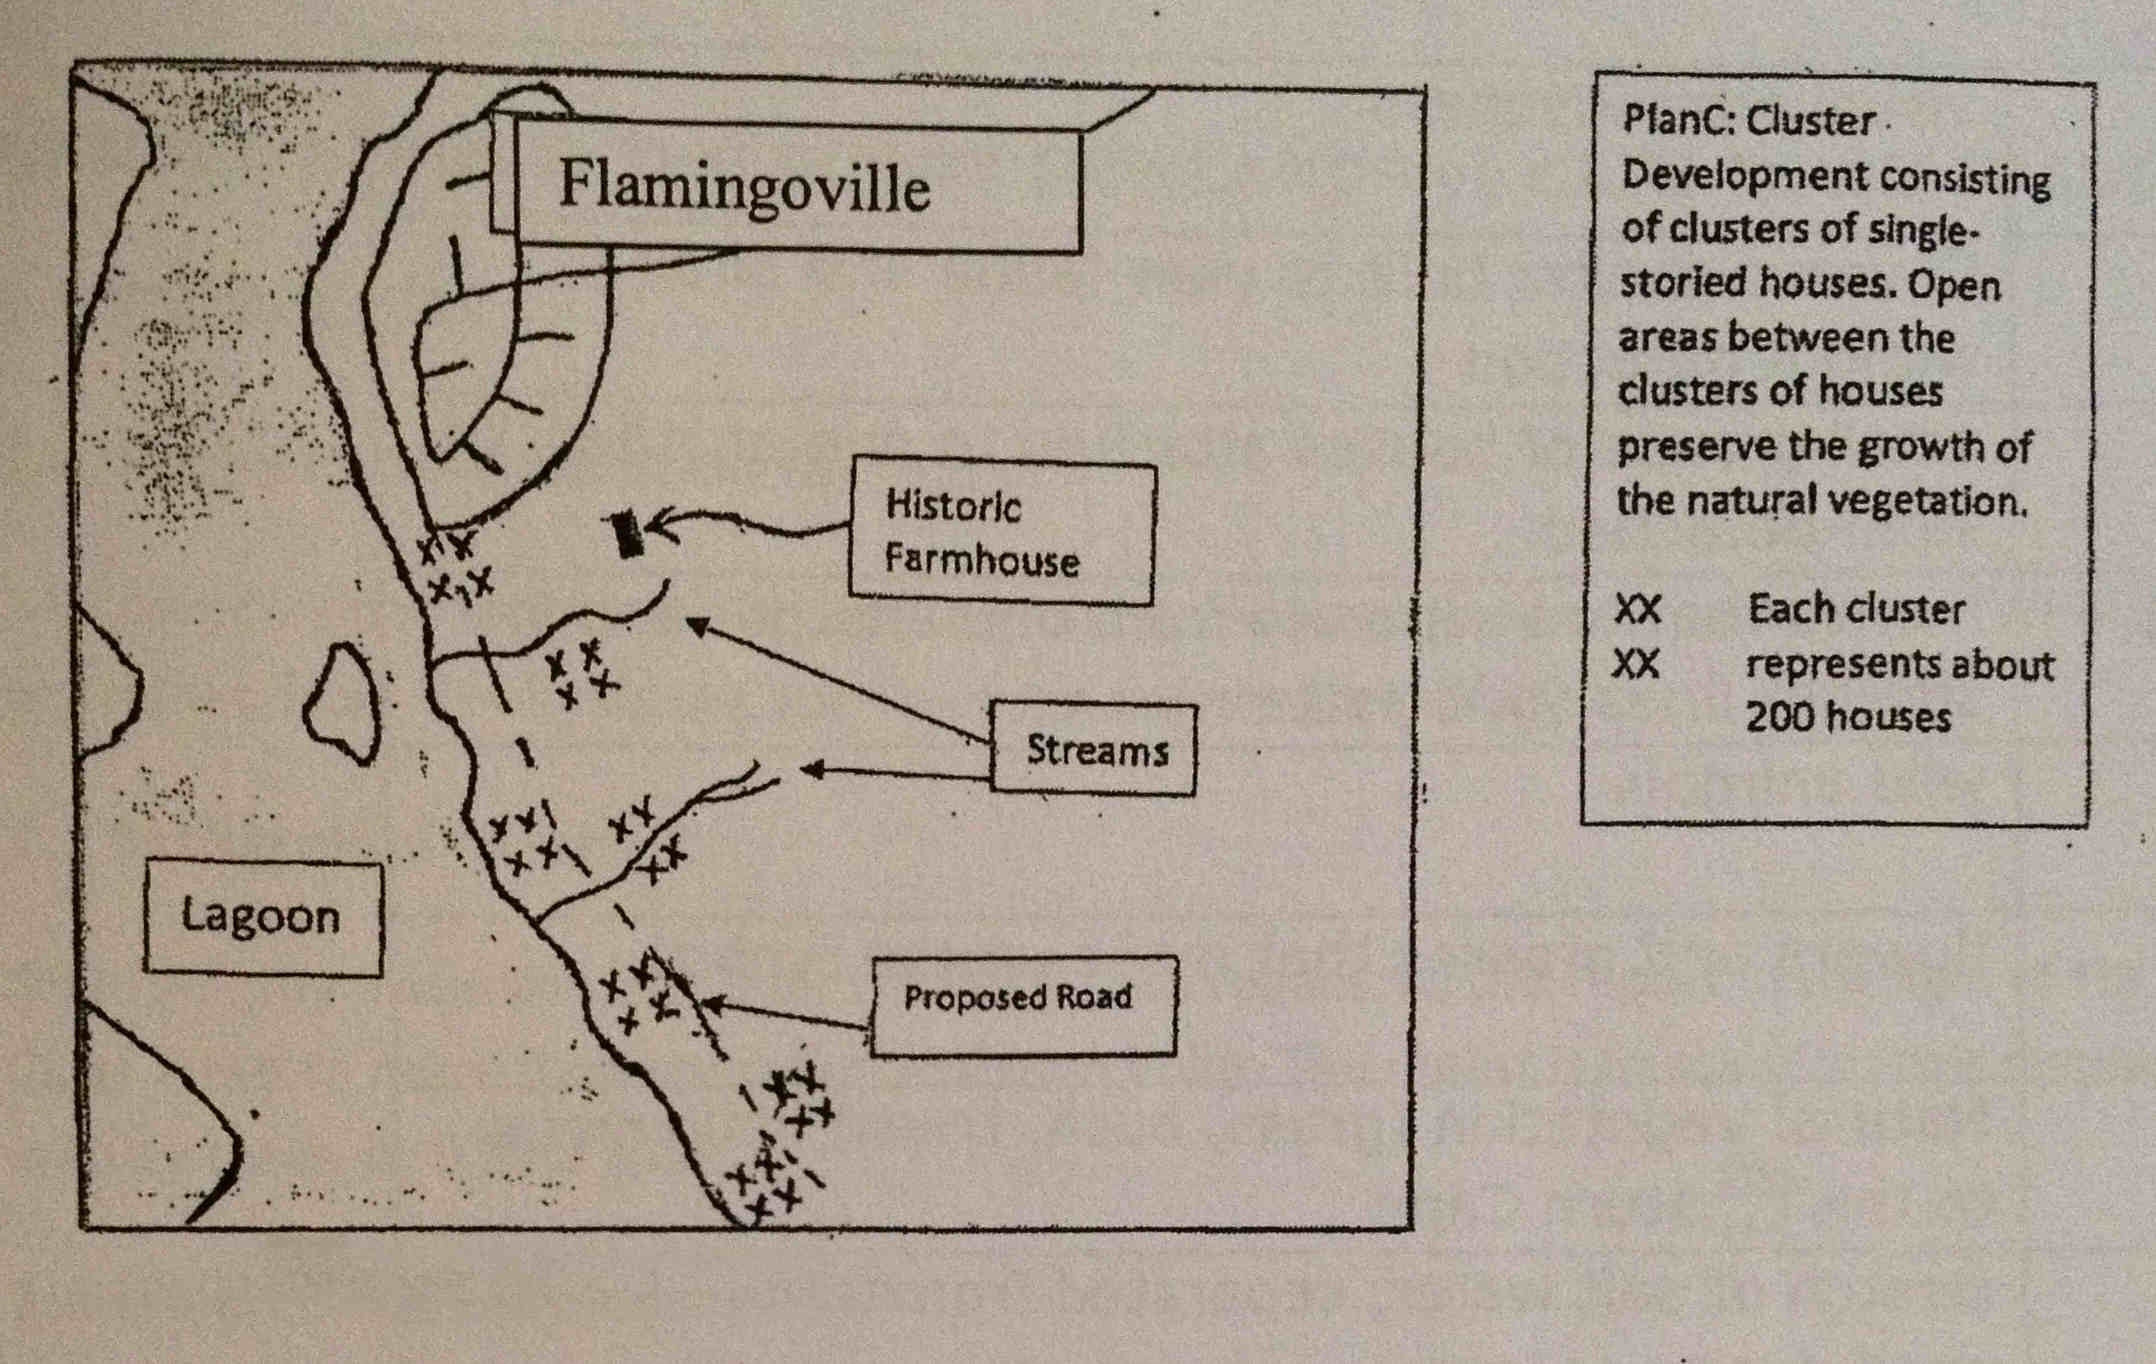
\includegraphics[width=0.6\textwidth]{plan_c}
	\caption{Map of plan C}
\end{figure}

\subsection{Effect on marine life}
\subsubsection{Effect}
\begin{itemize}
	\item A large portion of the lagoon is exposed to development.
	\item Both stream are exposed to development.
\end{itemize}

\subsubsection{Counter measures}
\begin{itemize}
	\item Water retention dams will be constructed to minimize pollution and maintain ecology.
\end{itemize}

\subsection{Economic impact}
\begin{itemize}
	\item The average distance from each house to the center of town is relatively high.
	\item This high distance drives up costs of infrastructure.
\end{itemize}

\subsection{Visual impact}
\begin{itemize}
	\item Only single story houses will be constructed.
	\item Development is not near historic farmhouse.
	\item Open areas between housing clusters.
\end{itemize}

\newpage
\section{CONCLUSIONS}
In the light of the above findings, the following conclusions have been drawn:

\subsection{Adequate environmental mitigation strategies}
Water retention dams will ensure that pollution in streams is contained and treated, as well as maintain the nearby ecology.

\subsection{Low cost to marine life}
Plan B has been determined to have the lowest cost to marine life. This is due to the fact that plan B exposes only one stream to development. Plan B also has the least amount of lagoon cost line exposed to development. Because of the condensed layout of plan B, traffic into the town along the proposed road will be contained, further minimizing the impact on wildlife.

\subsection{Low visual impact}
The plan with the lowest visual impact is plan B. Plan B condenses development perpendicularly to the proposed road and so visibility from the road is maximized.

\subsection{Low economic costs}
The plan with the lowest economic costs is plan B. Due to the layout of the development, infrastructure costs will be minimized.

\newpage
\section{RECOMMENDATIONS}
In light of the above conclusions, the following recommendations are made:

\subsection{Implement development plan B}
Plan B offers the lowest cost to marine life, has the lowest visual impact and has low economic costs.

\newpage
\listoffigures

\newpage
\section*{Glossary}
\textbf{Aesthetics} \quad visual attractiveness\\
\textbf{Bird Hide} \quad covered shelter built to view fauna and birds without detection\\
\textbf{Fynbos} \quad Natural vegetation indigenous to the Western Cape

\newpage
\printbibliography

\end{document}